% ============================================================
%  CHAPTER 4 — Segmentation-Guided Attention for RSVQA
% ============================================================
% To include in main.tex use:  \input{chapter4}
% Paper source: IGARSS 2024 — Tosato*, Boussaid* et al.
%
% Required packages in main.tex preamble:
%   \usepackage{booktabs}
%   \usepackage{tabularx}
%   \usepackage{multirow}
%   \usepackage{array}
% ============================================================

\chapter{Segmentation-Guided Attention for Remote Sensing Visual Question Answering}
\label{chap:seg_attention}
\startcontents[chapters]

\printmyminitoc{
	%\lipsum[1]
\textit{Chapter summary.} Standard RSVQA attention mechanisms compute attention weights directly from raw visual features, forcing the model to jointly discover relevant semantic categories and their spatial extent from supervision alone. This chapter instead guides attention with an explicit, multi-channel segmentation prior: a frozen UPerNet/Swin Transformer module, trained on 16 BD TOPO object classes, produces per-class spatial maps that condition attention jointly with the question. Evaluated on a preliminary TAMMI dataset over four Île-de-France departments, the proposed model improves overall accuracy by approximately 10\% over a no-attention baseline and 5\% over vanilla attention.
}
% ============================================================
\section{Introduction}
\label{sec:chap4_intro}
% ============================================================

The previous chapter addressed the generalization problem
in RSVQA from a data perspective, showing that LLM-based
question augmentation can improve model robustness to
unseen phrasings. However, data diversity alone does not
address a more fundamental limitation: the capacity of the
model to correctly identify and locate the visual content
relevant to a given question. In dense remote sensing scenes,
where multiple object classes coexist at varying scales and
spatial configurations, standard visual encoders tend to
produce globally averaged representations that fail to capture
the fine-grained spatial structure required for accurate
question answering. This chapter addresses this limitation
from an architectural perspective, proposing a method that
explicitly guides the model's visual attention using semantic
segmentation.

Attention mechanisms have become a cornerstone of visual
question answering pipelines. By weighting different spatial
regions of the visual feature map according to their relevance
to the input question, attention allows the model to
selectively focus on the parts of the image most informative
for answering. This has been shown to consistently improve
performance in general VQA~\cite{zhang2020context,
wei2020multimodality}, and has been adapted to the RSVQA
setting by~\cite{zheng2021mutual}, who propose a mutual
attention inception network that aligns spatial positions
with question words. However, existing attention mechanisms
in RSVQA operate directly on raw visual features, without
any explicit semantic understanding of the scene content.
In the context of remote sensing, where the visual appearance
of object classes (roads, buildings, vegetation, water areas)
is highly variable across regions, this lack
of semantic grounding limits the precision with which
attention can localize the relevant content.

Semantic segmentation provides exactly the kind of
structured, class-level understanding of the scene that
raw visual features lack. By explicitly identifying which
pixels belong to which object class, a segmentation map
encodes a rich spatial layout of the image that is directly
aligned with the semantic content of RSVQA questions,
which almost always refer to specific object classes
(\textit{e.g.}, \textit{``Is there a road?''}, \textit{``What
is the area of the water zone?''}). In the natural image
domain, segmentation has been used to guide attention in
VQA~\cite{gan2017vqs} and to produce faithful visual
explanations~\cite{wu2018faithful}. To the best of our
knowledge, however, this approach had not been explored in
the remote sensing VQA literature at the time of this work.

In this chapter, we propose to embed a segmentation-guided
attention mechanism into a RSVQA pipeline. A key original
aspect of this design is the use of \textit{multi-channel}
segmentation maps, one binary channel per object class,
rather than the traditional single-channel segmentation in
which each pixel receives a single class label. This choice
is motivated by the frequent spatial overlap between object
classes in remote sensing imagery (\textit{e.g.}, a road
passing through a vegetation zone), which a single-channel
representation cannot capture but which a multi-channel one
represents naturally, as detailed in
Section~\ref{sec:chap4_seg_multichannel}. The segmentation
itself is performed by a UPerNet model with a Swin
Transformer backbone~\cite{liu2021swin}, trained on 16
object classes derived from the BD TOPO geographic
database~\cite{bdtopo} and then kept frozen during VQA
training. The resulting 16-channel segmentation maps are
used to guide the computation of attention weights jointly
with the question representation, providing the model with
an explicit semantic prior over the spatial
layout of the scene that raw visual features alone do not
supply. We evaluate this approach on a new
dataset built from very high resolution airborne imagery
(BD ORTHO~\cite{bdortho}) over four
departments of the Île-de-France region, which constitutes
a preliminary version of the TAMMI dataset introduced in
full in Chapter~\ref{chap:tammi}. Our ablation study
demonstrates gains of approximately 10\% in overall
accuracy over a baseline without attention, and 5\% over
a vanilla attention mechanism without segmentation guidance.

The remainder of this chapter is organized as follows.
Section~\ref{sec:chap4_rw} reviews related work on
attention mechanisms and segmentation-guided approaches
in VQA. Section~\ref{sec:chap4_dataset} describes the
dataset and segmentation annotations used in this work.
Section~\ref{sec:chap4_method} presents the proposed
architecture. Section~\ref{sec:chap4_experiments} details
the experimental results and ablation study.
Section~\ref{sec:chap4_conclusion} concludes with
limitations and perspectives.

% ============================================================
\section{Related Work}
\label{sec:chap4_rw}
% ============================================================
% Scope: specific to this contribution only.
% General VQA task definition, RS background, and broad
% vision-language architectures are in Ch. 2.
% Ch. 3 already covered data augmentation and linguistic bias.
% Here: attention in VQA, segmentation-guided vision, RSVQA attention.
This section reviews the two bodies of work this chapter connects. 
Section~\ref{sec:chap4_rw_attention} reviews attention mechanisms 
in VQA generally and in RSVQA specifically, where attention is computed 
directly from raw visual features. Section~\ref{sec:chap4_rw_seg} then reviews work that instead guides attention with an explicit 
semantic segmentation prior, established in the natural image domain but, at the time of this work, unexplored in RSVQA.
\subsection{Attention Mechanisms in Visual Question Answering}
\label{sec:chap4_rw_attention}

Attention mechanisms were introduced in VQA to address a
key limitation of early models, which represented an
entire image with a single global feature vector,
regardless of the question being asked.
\textcite{yang2016stacked} propose Stacked Attention
Networks (SAN), which use the semantic representation of
the question as a query to iteratively search for
relevant image regions, performing multiple steps of
attention to progressively refine the focus of the model.
\textcite{anderson2018bottomup} further refine this idea with
a bottom-up and top-down attention mechanism, in which a
bottom-up module (based on Faster R-CNN) proposes
object-level image regions, while a top-down mechanism
determines which of these regions are relevant to the
question. This object-centric formulation of attention
became a standard component of VQA architectures, as it
aligns naturally with the object-oriented phrasing of most
questions.

In the RSVQA setting, \textcite{zheng2021mutual} propose a
mutual attention inception network that computes attention
weights by modeling the alignment between spatial image
positions and question words, using an inception-based
visual backbone. This work demonstrates that attention
improves performance on RSVQA benchmarks, in a manner
consistent with findings in the natural image domain.
However, in the approaches discussed above,
including those applied to remote sensing, attention
weights are computed directly from raw visual features,
without any explicit intermediate representation of the
scene's semantic content. The attention mechanism must
therefore implicitly learn both \textit{what} the relevant
semantic categories are and \textit{where} they are
located, from the VQA supervision signal alone. This
joint demand is particularly challenging in remote
sensing imagery, where object classes are visually
ambiguous at a given resolution and the training signal
for any single question type is comparatively sparse.

\subsection{Segmentation as a Prior for Visual Reasoning}
\label{sec:chap4_rw_seg}

An alternative line of work proposes to decouple these two
demands by providing the attention mechanism with an
explicit semantic segmentation of the scene, computed as
a separate task. \textcite{gan2017vqs} introduce the VQS
dataset, which links segmentation annotations to
question-answer pairs, and show that supervising attention
with segmentation masks improves both VQA accuracy and
the interpretability of the resulting attention maps, while
also enabling question-focused semantic segmentation as a
complementary output. \textcite{wu2018faithful} pursue a
related goal from the perspective of explainability,
proposing a multimodal explanation framework in which
segmentation-derived attention maps are used to generate
visual justifications for predicted answers that are
faithful to the model's actual reasoning process, as
opposed to post-hoc visualizations that may not reflect
the features actually used for prediction.

Both lines of work demonstrate, in the natural image
domain, that segmentation provides a more informative and
more interpretable prior for attention than raw visual
features alone: it supplies the attention mechanism with
an explicit, class-level representation of the scene,
removing the need to jointly discover semantic categories
and their spatial extent from VQA supervision alone. To
the best of our knowledge, at the time of this work, this
strategy had not been explored in the remote sensing VQA
literature, despite the fact that remote sensing benefits
from a particularly rich source of segmentation-relevant
annotations through geographic databases such as BD
TOPO~\cite{bdtopo}. This chapter addresses this gap by
introducing a segmentation-guided attention mechanism for
RSVQA, using multi-channel segmentation maps derived from
such a geographic database as an explicit semantic prior.

% ============================================================
\section{Dataset and Segmentation Annotations}
\label{sec:chap4_dataset}
% ============================================================

\subsection{Very High Resolution Imagery}
\label{sec:chap4_dataset_vhr}

The experiments in this chapter are conducted on a
preliminary version of the TAMMI dataset, introduced in
full in Chapter~\ref{chap:tammi}. We provide here a concise
overview of the data used.

The visual inputs consist of very high resolution (VHR)
airborne RGB orthophotos from the BD ORTHO
database~\cite{bdortho}, produced by the French National
Geographic Institute (IGN) at a ground resolution of 20\,cm.
The images are subdivided into patches of
$1000 \times 1000$ pixels, each covering an area of
$200\,\text{m} \times 200\,\text{m}$ on the ground. We
select four adjacent departments from the Île-de-France
region (Paris, Hauts-de-Seine, Val-de-Marne, and
Seine-Saint-Denis) resulting in 16,274 patches. The
dataset is split into training (60\%), validation (20\%),
and test (20\%) sets, with the same split applied to both
the segmentation task and the VQA task.

\subsection{Segmentation Annotations from BD TOPO}
\label{sec:chap4_dataset_seg}

A key characteristic of this dataset, and the aspect most
directly relevant to the contribution of this chapter, is
the availability of dense segmentation annotations derived
from the BD TOPO database~\cite{bdtopo}, a vectorial
description of the French territory maintained by IGN.

\subsubsection{Class taxonomy}
\label{sec:chap4_seg_classes}

We define 16 segmentation classes organized into six
thematic groups, reflecting the semantic categories most
relevant to RSVQA questions over urban and peri-urban
areas:

\begin{itemize}
    \item \textbf{Buildings:} Building, Cemetery, Sports
    Field, Water Tank, Pylon, Surface Construction;
    \item \textbf{Land Use:} Foreshore Zone, Vegetation
    Zone;
    \item \textbf{Water Area;}
    \item \textbf{Transport:} Airfield, Transportation
    Construction, Road, Railway;
    \item \textbf{Regulated Areas:} Public Forest,
    National Park;
    \item \textbf{Services and Activities:} Museums,
    Monuments, Schools, and similar entities.
\end{itemize}

The choice of 16 classes reflects a trade-off between
semantic richness and annotation density: finer-grained
taxonomies would yield sparser annotations in urban areas,
while coarser ones would lose the class-level specificity
required to guide attention toward the objects referenced
in RSVQA questions.

\subsubsection{Multi-channel segmentation}
\label{sec:chap4_seg_multichannel}

A critical design choice in this work is the use of
\textit{multi-channel} segmentation maps rather than the
traditional single-channel representation. In standard
semantic segmentation, each pixel is assigned a single
class label, which implicitly assumes that object classes
do not overlap spatially. This assumption is frequently
violated in remote sensing imagery, where objects from
different classes can occupy the same pixel footprint at
the given resolution (\textit{e.g.}, a road passing through
a vegetation zone, or a building adjacent to a water area).

Our multi-channel representation instead produces one
binary channel per class, where each channel independently
indicates the presence or absence of that class at each
spatial location. This allows overlapping object classes
to be represented simultaneously, providing a richer and
more faithful description of the scene layout. Concretely,
the segmentation output $f_\text{seg} \in \mathbb{R}^{16
\times H \times W}$, with $H = W = 1000$ matching the
$1000 \times 1000$ pixel resolution of the input VHR patch
$p_\text{VHR}$ (Section~\ref{sec:chap4_dataset_vhr}), encodes the full spatial distribution
of all 16 classes over the image, which is then used
directly to guide the attention computation.

\subsubsection{Segmentation module training}
\label{sec:chap4_seg_training}

The segmentation module consists of a UPerNet
architecture~\cite{xiao2018upernet} with a Swin
Transformer backbone~\cite{liu2021swin}, pre-trained on
the ADE20K dataset~\cite{zhou2019ade20k}, a large-scale
semantic segmentation benchmark of roughly 25,000 natural
images annotated with 150 object and stuff categories
spanning indoor and outdoor scenes. While ADE20K's imagery
and class taxonomy differ substantially from remote sensing,
pre-training on it still provides the backbone with
general-purpose visual features, rather than
starting from randomly initialized weights. A convolutional
layer is added to map the feature maps $f_\text{seg}$ to
the 16-channel output, which is then bilinearly interpolated
to the spatial resolution of the input patch $p_\text{VHR}$.

We fine-tune this segmentation module on the 16-class
annotations described above, using the same training split
as the VQA task. After training, the weights of the
segmentation module are \textbf{frozen} before the VQA
pipeline is trained. This design choice is motivated by two
considerations. First, freezing the segmentation module
ensures that the attention mechanism learns to exploit the
semantic layout produced by segmentation rather than
co-adapting with it, which would risk collapsing the
segmentation representations toward features that are
useful for VQA but not necessarily semantically meaningful.
Second, it decouples the two training objectives, making
the overall pipeline more stable and interpretable.

\subsection{Question/Answer Pairs}
\label{sec:chap4_dataset_qa}

The dataset contains 146,848 question/answer pairs
distributed across nine question types organized into
four categories, summarized in Table~\ref{tab:chap4_qtypes}.
Questions are generated automatically from the BD TOPO
annotations following a two-stage procedure designed to
balance both question type and answer type distributions,
reducing language biases~\cite{chappuis2025langbias}. Question
type is balanced first, by randomly generating ten questions
per question type for each VHR patch $p_\text{VHR}$. Answer
type is then balanced by defining, for each question type, a
maximum number of questions per answer type, $N_{Q,A}$; only
questions whose answer type is less represented than
$N_{Q,A}$ are retained. To reach a sufficient number of
questions under this filtering, the VHR patches are browsed
twice. The full
question generation methodology is described in
Chapter~\ref{chap:tammi}.

\begin{table}[ht]
\centering
\small
\caption{Question type taxonomy used in the dataset.
Nine question types are organized into four categories.
Abbreviations used in Table~\ref{tab:chap4_results}
are shown in parentheses.}
\label{tab:chap4_qtypes}
\begin{tabularx}{\textwidth}{l >{\raggedright\arraybackslash}X}
\toprule
\textbf{Category} & \textbf{Question types} \\
\midrule
Class questions & Presence, Count, Density \\
Object questions & Absolute location, Area \\
Two-class questions & Comparison \\
Object relation questions & Relative location, Distance,
                            Nearest object \\
\bottomrule
\end{tabularx}
\end{table}

The distribution of answers across question types is
illustrated in Figure~\ref{fig:chap4_dist}. Each sector
of the chart corresponds to one question type, and the
inner ring shows the distribution of answers within that
type. For numerical answers (count, area, distance), only
the ordering is shown without explicit labeling, with
maximum values of 280 (count), 40,000\,m$^2$ (area), and
273\,m (distance). The chart confirms that the balancing
procedure successfully avoids extreme answer skew within
each question type, which is critical for training models
that are robust to linguistic bias.

\begin{figure}[ht]
    \centering
    % NOTE: insert Figure 1 from the paper here
    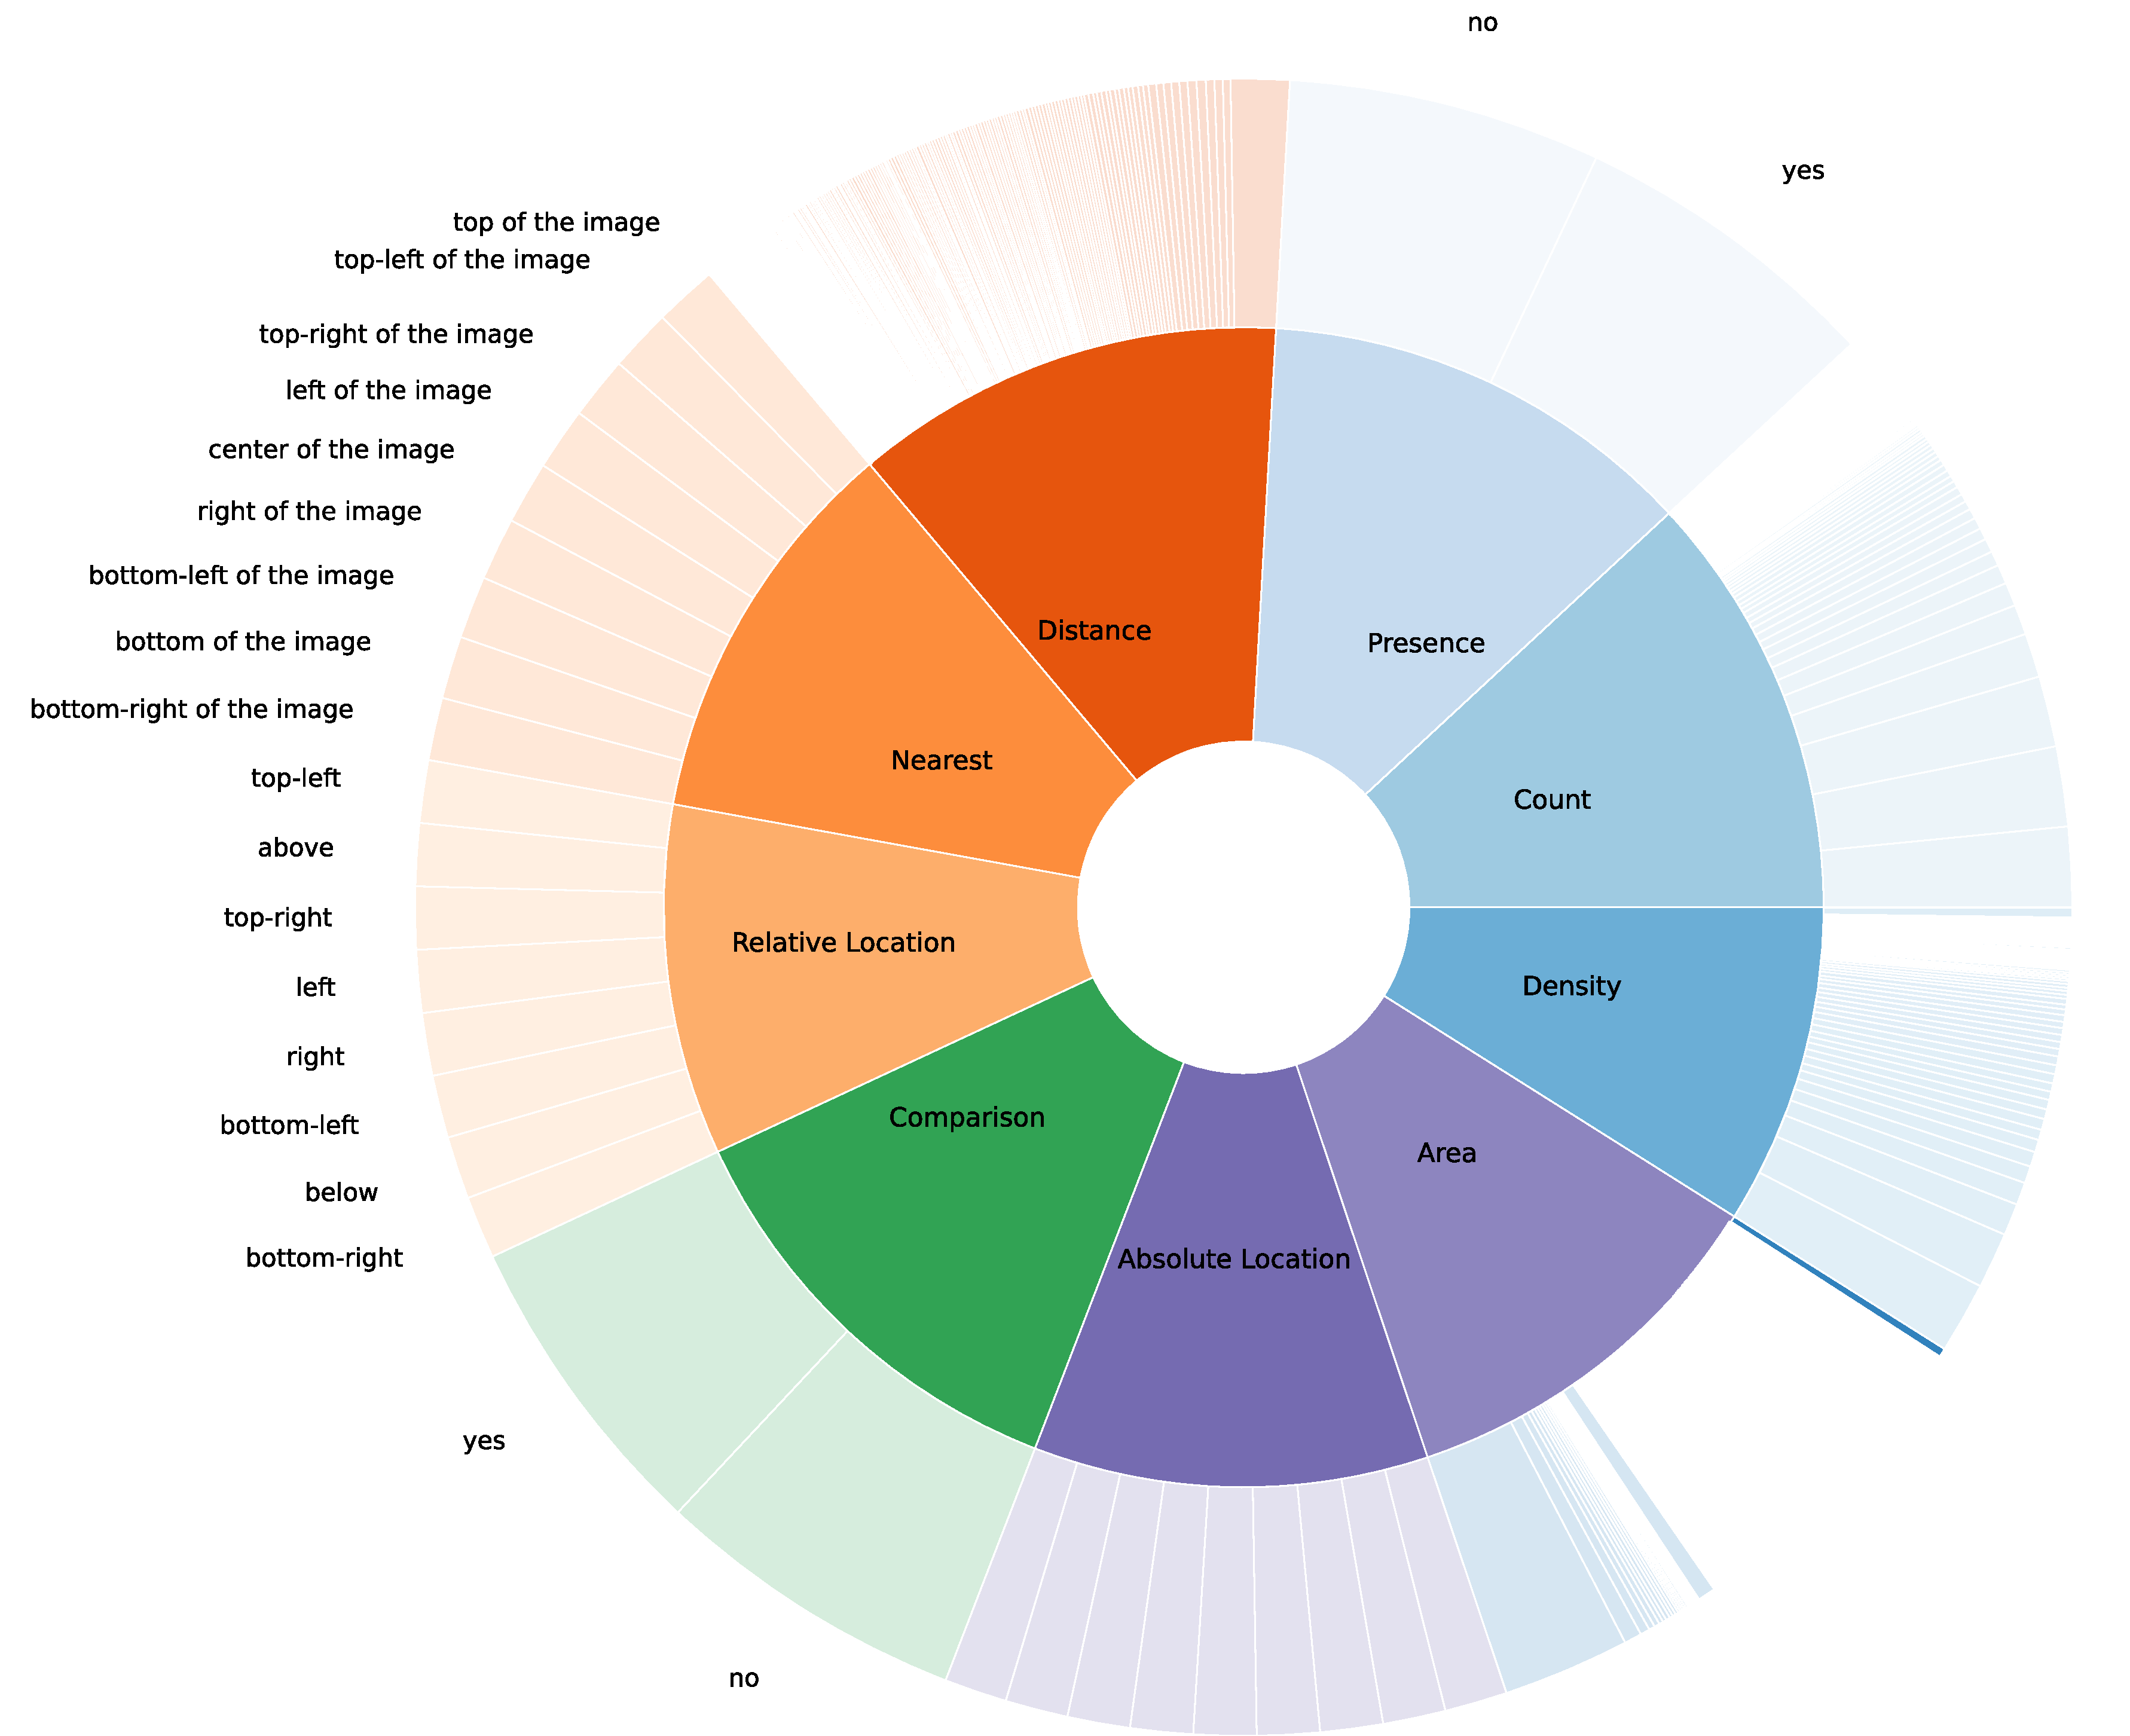
\includegraphics[width=0.7\textwidth]{images/Seg/newtry.pdf}
    \caption{Distribution of answers by question type.
    Numerical answer labels are omitted and shown in
    order only. Maximum values: 280 (count), 40,000\,m$^2$
    (area), 273\,m (distance). The balanced distribution
    across answer types within each question category
    reduces language bias during training.}
    \label{fig:chap4_dist}
\end{figure}

% ============================================================
\section{Segmentation-Guided Attention Architecture}
\label{sec:chap4_method}
% ============================================================
This section presents the proposed architecture in four parts: Section~\ref{sec:chap4_method_overview} gives a high-level overview of the full pipeline, Section~\ref{sec:chap4_method_features} details the frozen visual and textual feature extractors, Section~\ref{sec:chap4_method_attention} presents the segmentation-guided attention module itself, and Section~\ref{sec:chap4_method_prediction} describes the prediction head and training procedure.
\subsection{Overview}
\label{sec:chap4_method_overview}

We introduce a RSVQA pipeline that incorporates
segmentation as an explicit prior for the attention
mechanism. The pipeline takes as input a VHR patch
$p_\text{VHR}$ and a natural language question $q$, and
produces a predicted answer from a closed vocabulary of
1,000 classes. It consists of three components: a feature
extraction module, a segmentation-guided attention module,
and a prediction head. Figure~\ref{fig:chap4_arch}
illustrates the full architecture.

 \begin{figure}[ht]
   \centering
   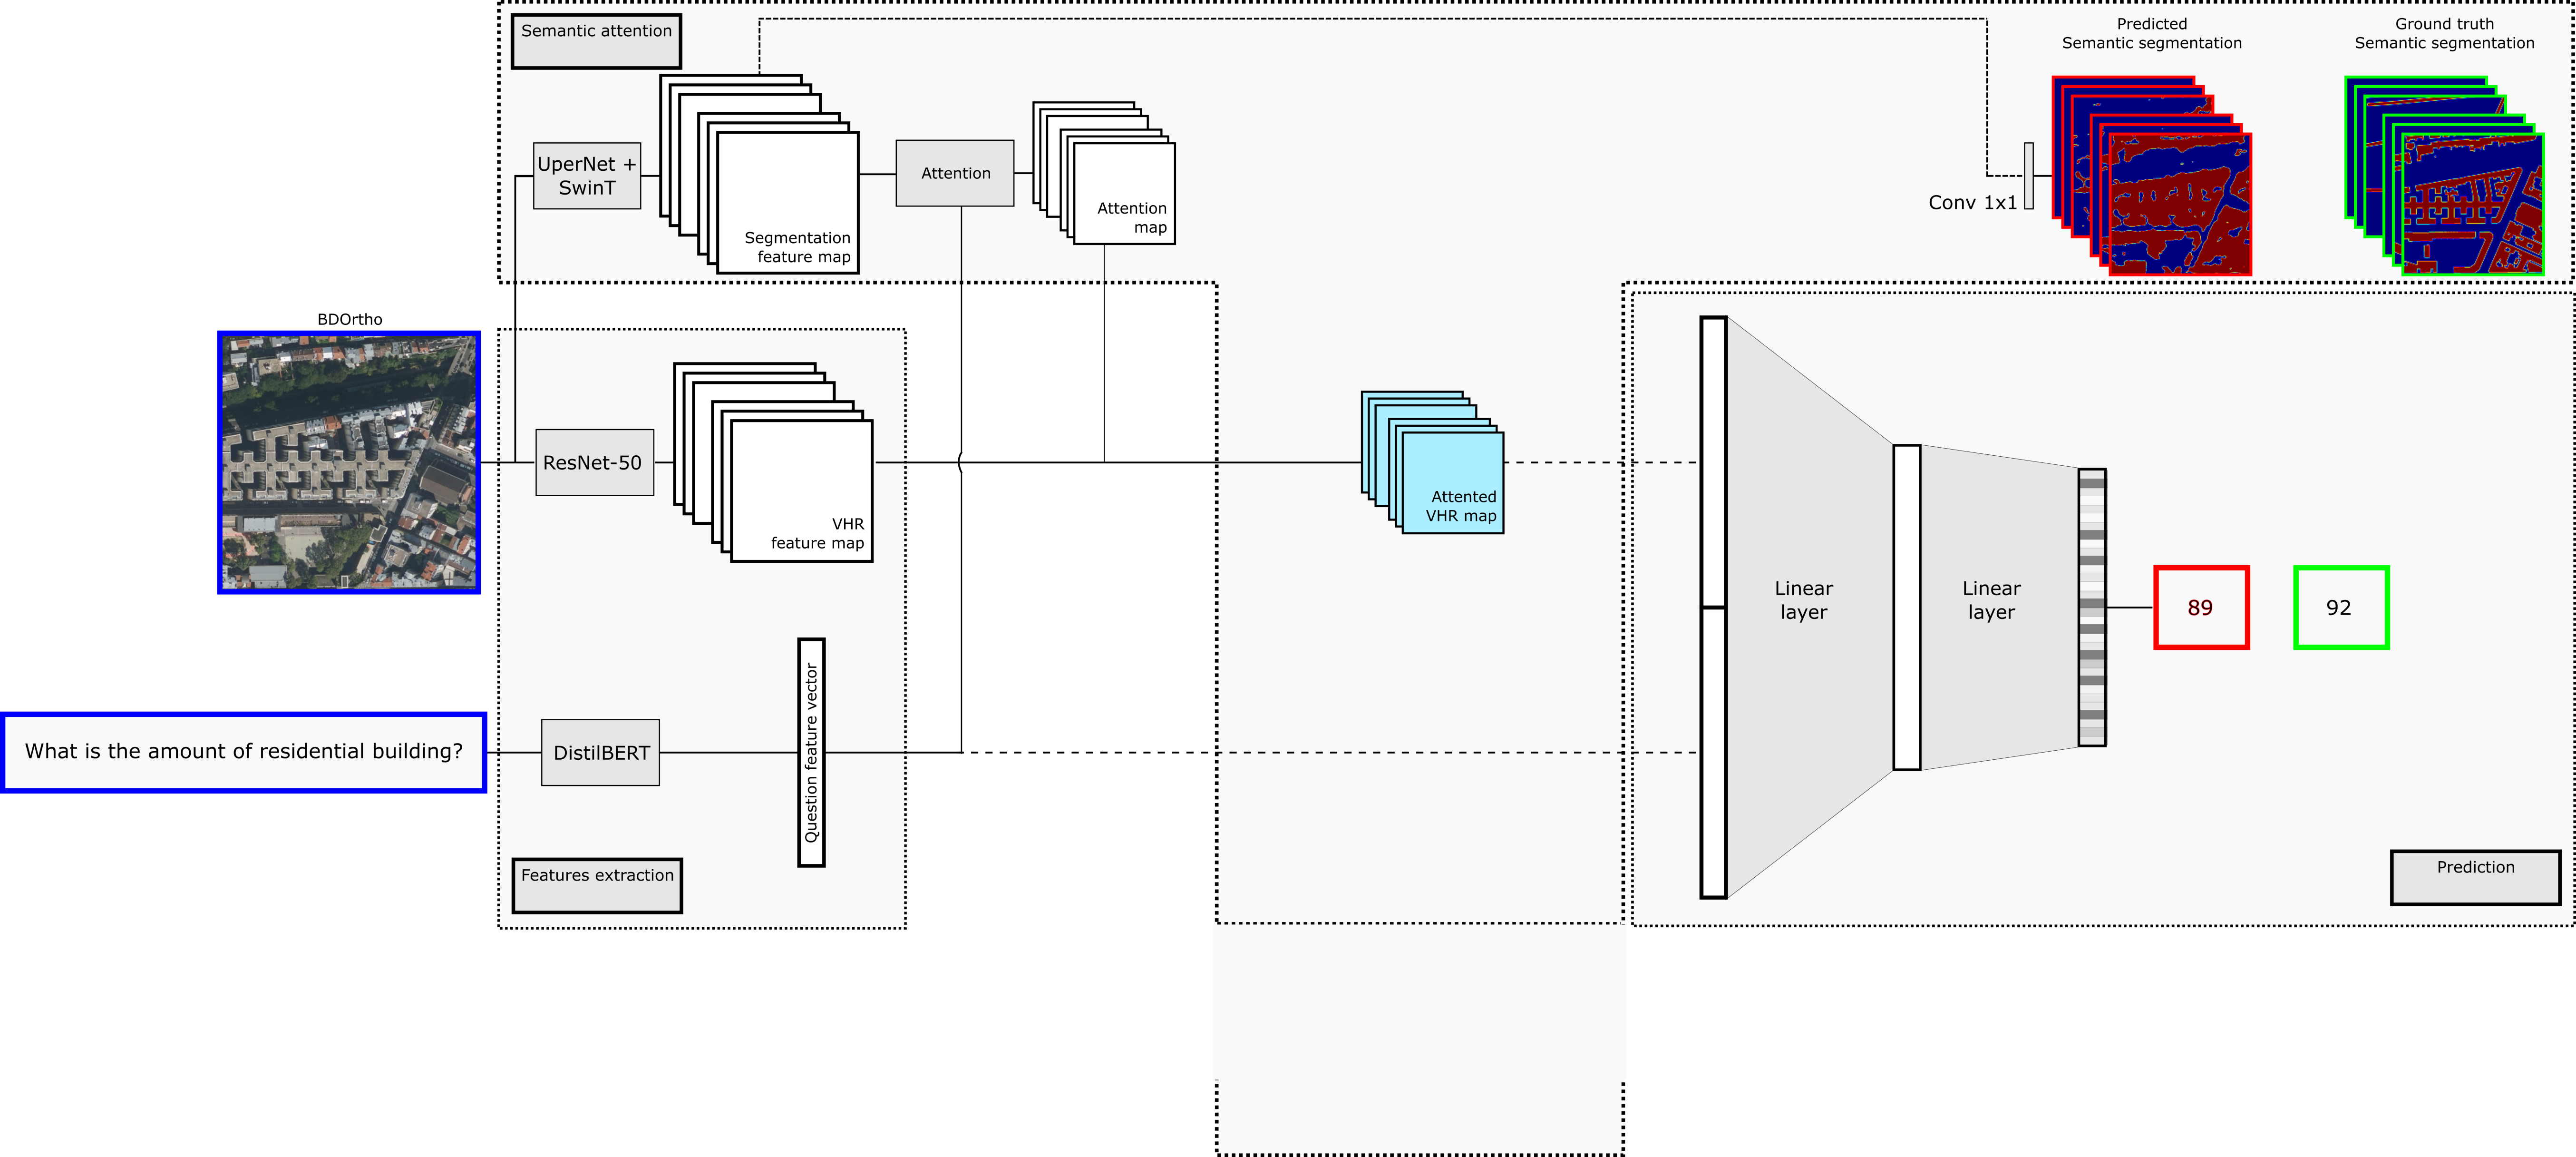
\includegraphics[width=\textwidth]{images/Seg/model1_1.png}
   \caption{Architecture of the proposed segmentation-guided
   attention pipeline. Inputs (VHR image and question) are
   shown in blue; outputs (answer prediction and segmentation)
   in red; ground truths in green.}
   \label{fig:chap4_arch}
 \end{figure}

\subsection{Feature Extraction}
\label{sec:chap4_method_features}

\textbf{Visual features.} Visual features $f_\text{VHR}$
are extracted from the VHR patch using a ResNet-50
model~\cite{he2016resnet} pre-trained on ImageNet, from
which the final fully-connected layer is removed. The
ResNet-50 weights are kept frozen throughout training.
The choice of ResNet-50 over larger variants is
deliberate: rather than relying on a more powerful visual
backbone to compensate for the lack of semantic grounding,
this work shows that even with a comparatively modest
encoder, explicitly guiding attention with segmentation
yields improvements. ResNet-50 remains a
strong and widely-used baseline in its own right.

\textbf{Textual features.} Textual features $f_q$ are
extracted from the question $q$ using a DistilBERT
encoder~\cite{sanh2019distilbert}, also kept frozen. The
use of frozen encoders for both modalities ensures that
the training signal is directed toward the attention and
fusion modules rather than toward refining the base
representations, which stabilizes the learning process
given the relatively modest size of the dataset.

\subsection{Segmentation-Guided Attention}
\label{sec:chap4_method_attention}

The segmentation-guided attention module computes a
spatial attention map $\mathbf{a}$ that is applied to the
visual features $f_\text{VHR}$, emphasizing regions
relevant to the question. The computation proceeds as
follows.

The textual features $f_q$ are projected to a
250-dimensional space via a linear layer with dropout
$d = 0.5$:

\begin{equation}
    \tilde{f}_q = \text{Dropout}(W_q f_q + b_q),
    \quad \tilde{f}_q \in \mathbb{R}^{250}
\end{equation}

Simultaneously, the segmentation feature map
$f_\text{seg} \in \mathbb{R}^{16 \times H \times W}$ is
projected to a 250-channel spatial representation via a
$1 \times 1$ convolution with dropout $d$:

\begin{equation}
    \tilde{f}_\text{seg} = \text{Dropout}(\text{Conv}_{1
    \times 1}(f_\text{seg})),
    \quad \tilde{f}_\text{seg} \in \mathbb{R}^{250 \times
    H \times W}
\end{equation}

The two representations are concatenated along the channel
dimension (broadcasting $\tilde{f}_q$ spatially), and a
ReLU activation followed by a $1 \times 1$ convolution
produces a single-channel attention glimpse:

\begin{equation}
    \mathbf{a} = \text{Conv}_{1 \times 1}\left(
    \text{ReLU}\left([\tilde{f}_q \oplus
    \tilde{f}_\text{seg}]\right)\right),
    \quad \mathbf{a} \in \mathbb{R}^{1 \times H \times W}
\end{equation}

The attention map $\mathbf{a}$ is then applied element-wise
to the visual features:

\begin{equation}
    \hat{f}_\text{VHR} = \mathbf{a} \odot f_\text{VHR}
\end{equation}

The key insight of this design is that the attention weights
are conditioned on \textit{both} the question semantics
(via $\tilde{f}_q$) and the spatial class layout (via
$\tilde{f}_\text{seg}$). This allows the model to focus
on image regions that are simultaneously relevant to the
question and semantically coherent, for instance,
attending to road pixels when answering a question about
roads, rather than activating on arbitrary high-contrast
regions.

\subsection{Prediction Head and Training}
\label{sec:chap4_method_prediction}

The attended visual features $\hat{f}_\text{VHR}$ are
concatenated with the textual features $f_q$ to form a
global multimodal representation. This is passed through
a 2-layer MLP with ReLU activations and dropout $d$,
producing a 1,000-dimensional output corresponding to the
1,000 most frequent answers in the training set.

The model is trained end-to-end (excluding the frozen
encoders and segmentation module) using a cross-entropy
loss, optimized with Adam at a learning rate of $10^{-6}$
and a batch size of 4. Training runs for approximately
100 hours on a single NVIDIA V100-16G GPU.

% ============================================================
\section{Experimental Study}
\label{sec:chap4_experiments}
% ============================================================
This section evaluates the proposed architecture in two stages. 
Section~\ref{sec:chap4_seg_results} first evaluates the segmentation module on its own,
 since the quality of the semantic prior it provides directly bounds what segmentation-guided attention can achieve downstream. 
 Section~\ref{sec:chap4_vqa_results} then evaluates the full VQA pipeline against two ablations, 
isolating the respective contributions of attention and of segmentation guidance specifically.
\subsection{Segmentation Results}
\label{sec:chap4_seg_results}

The segmentation module is evaluated independently on the
validation set using a precision-recall curve with 20
thresholds, identifying the optimal per-class threshold.
The model achieves an overall precision of 53.6\%, an
overall recall of 73.2\%, and an overall F1-score of
60.1\% on the test set. The relatively higher recall than precision
reflects the characteristics of the multi-channel
formulation: since each channel independently detects
one class, the model tends toward inclusive detection
(fewer missed objects) at the cost of some false
positives. These results confirm that the segmentation
module produces meaningful spatial class maps, providing
a reliable semantic prior for the attention mechanism.

While an F1-score of 60.1\% would be modest as a
standalone segmentation benchmark for 16-class land cover
classification, the goal of this module is not to achieve
state-of-the-art segmentation but to provide a sufficiently
informative semantic prior for the attention mechanism.
As shown in Section~\ref{sec:chap4_vqa_results}, even at
this level of quality, the segmentation maps yield a
measurable improvement in VQA accuracy, indicating that
the attention mechanism is able to extract useful spatial
and semantic structure from imperfect segmentation
predictions.

\subsection{VQA Results and Ablation Study}
\label{sec:chap4_vqa_results}

Table~\ref{tab:chap4_results} presents the per-question
type accuracy, overall accuracy (OA), and average accuracy
(AA) for the proposed model and two ablation variants:

\begin{itemize}
    \item \textbf{Proposed}: full model with
    segmentation-guided attention;
    \item \textbf{A1}: vanilla attention without
    segmentation guidance;
    \item \textbf{A2}: no attention mechanism.
\end{itemize}

\begin{table}[ht]
\centering
\small
\begin{tabular}{l ccc}
\toprule
\multirow{2}{*}{\textbf{Question type}}
  & \textbf{Proposed} & \textbf{A1} & \textbf{A2} \\
  & (Attention + Segmentation) & (Attention only) & (No attention) \\
\midrule
Presence & \textbf{89.36} & 85.79 & 80.94 \\
Count & \textbf{26.36} & 22.98 & 10.50 \\
Density & \textbf{23.42} & 20.99 & 20.38 \\
Absolute location & \textbf{14.61} & 13.82 & 12.96 \\
Area & \textbf{56.98} & 44.69 & 40.94 \\
Comparison & \textbf{93.08} & 82.94 & 74.00 \\
Relative location & \textbf{13.76} & 11.91 & 13.41 \\
Distance & \textbf{74.19} & 74.19 & 59.80 \\
Nearest object & \textbf{17.21} & 15.60 & 13.44 \\
\midrule
Average Accuracy (AA) & \textbf{43.24} & 39.40 & 34.91 \\
Overall Accuracy (OA) & \textbf{45.44} & 41.43 & 36.26 \\
\bottomrule
\end{tabular}
\caption{VQA results for the proposed model and ablation
studies. All values are accuracy percentages.
Best results in \textbf{bold}.}
\label{tab:chap4_results}
\end{table}

\subsection{Discussion}
\label{sec:chap4_discussion}

\textbf{Effect of segmentation-guided attention.}
The proposed model outperforms both ablation variants
across all question types. The gain over A2 (no attention)
is approximately 9\% in OA and 8\% in AA, confirming that
the attention mechanism provides a substantial benefit.
The additional gain over A1 (vanilla attention without
segmentation) is approximately 4\% in OA and 4\% in AA,
demonstrating that segmentation guidance provides a
meaningful improvement beyond attention alone. The
improvement is consistent across question types, suggesting
that the semantic prior introduced by segmentation benefits
a broad range of visual reasoning tasks rather than
being specific to a particular question category.

\textbf{Spatial reasoning questions.}
The lowest per-question type accuracies are observed for
question types involving spatial relationships: absolute
location (2a, 14.61\%), relative location (4a, 13.76\%),
and nearest object (4c, 17.21\%). This is consistent with
the inherent difficulty of spatial reasoning in end-to-end
deep learning models~\cite{cui2019multiscale}: recognizing
the class of an object and determining its position within
the image are distinct tasks that standard architectures
do not disentangle. The availability of segmentation maps
partially mitigates this limitation, but spatial reasoning
remains the primary failure mode of the model.

\textbf{Density vs. area questions.}
An interesting pattern emerges when comparing density
questions (1c, 23.42\%) with area questions (2b, 56.98\%).
Despite both involving quantitative reasoning about object
extent, density questions are significantly harder. Two
factors contribute to this gap. First, density predictions
are continuous values in $[0, 1]$, while area predictions
are positive integers, requiring higher precision from the
model. Second, density questions involve entire object
classes rather than individual objects, making the
prediction more sensitive to the global spatial
distribution of the class across the image.

\textbf{Comparison questions.}
The highest accuracy is achieved on comparison questions
(3, 93.08\%), which ask whether the count of one object
class is greater or less than another. This task is
relatively tractable because it reduces to a binary
classification over two class counts, and the segmentation
map directly provides class-level spatial information that
supports this comparison.

% ============================================================
\section{Conclusion and Limitations}
\label{sec:chap4_conclusion}
% ============================================================

In this chapter, we proposed a segmentation-guided
attention mechanism for RSVQA, arguing that the explicit
semantic layout provided by multi-channel segmentation
maps constitutes a more informative prior for visual
attention than raw visual features alone. We evaluated
this approach on a new dataset built from VHR airborne
imagery and BD TOPO annotations over four Île-de-France
departments. Our ablation study confirms that
segmentation-guided attention improves overall accuracy
by approximately 10\% over a no-attention baseline and
5\% over vanilla attention, with consistent gains across
all question types.

\textbf{Limitations.}
Several limitations should be acknowledged. First, the
dataset used in this chapter covers only four
departments of the Île-de-France region, limiting
geographic diversity. The extent to which the proposed
approach generalizes to other geographic regions, land
use patterns, or image resolutions remains an open
question. Second, the segmentation module is trained and
evaluated on the same geographic region as the VQA task,
which may introduce domain overlap between the two
tasks. Third, while Section~\ref{sec:chap4_seg_results} argues
that the segmentation module's F1-score of 60.1\% is
sufficient to provide a useful semantic prior, it remains
unclear whether further improvements in segmentation
quality would yield proportional gains in VQA accuracy,
or whether the attention mechanism already extracts most
of the available signal from the current segmentation
maps. Disentangling these two factors would require
training the VQA pipeline with segmentation modules of
varying quality, which is left for future work. Fourth, the attention mechanism produces a
single glimpse $\mathbf{a}$, which may be insufficient
for questions requiring reasoning over multiple spatially
distant regions simultaneously. %Fifth, the model operates
on VHR optical imagery only; the contribution of SAR
modality to segmentation-guided attention remains
unexplored at this stage.

\textbf{Perspectives.}
The results of this chapter motivate a natural extension,
addressed in the following chapter: the dataset is
extended to six departments and enriched with SAR and multispectral
imagery to produce the full TAMMI Dataset
(Chapter~\ref{chap:tammi}). More broadly, this chapter
demonstrates that auxiliary annotations (e.g., segmentation)
can provide supervision signals that
benefit the primary VQA task beyond what is available
from question-answer pairs alone, a principle that
recurs in different forms throughout the remaining
contributions of this thesis.

While this chapter demonstrated that \textit{what} the
model attends to can be significantly improved through
semantic segmentation, the following chapter turns to the
question of \textit{what data} the model is trained on,
introducing the complete TAMMI dataset, which extends and
completes the preliminary benchmark used here.

% ============================================================
% BIBLIOGRAPHY ENTRIES NEEDED FOR THIS CHAPTER
% (add to your main .bib file)
% ============================================================
%dép